\section{Managing Project Groups}
Before any project group can be useful it has to be created first.
Administrators need to have the ability to add, edit, and delete project groups.
The administration tools we provide have to be easy and fast to use, since they potentially have to be used many times.
This section describes how we implemented the administration tools needed to manage project groups.

The features we provide to manage project groups are known as administration tools in Moodle and can be accessed in the site administration menu as seen in \figref{fig:navigation}.

\begin{figure}[htb]
	\centering
		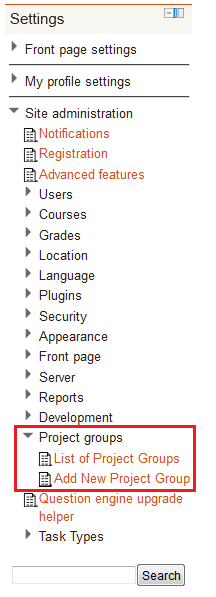
\includegraphics[scale=0.75]{images/admin-navigation.png}
	\morscaption{The settings block, which contains the site administration menu} 
	\label{fig:navigation}
\end{figure}

From here we provide a link to a list of all project groups and a link to a page, from where a new project group can be created.
